\section{Additional Data}
\subsection{US case data}

Interface amplitude, circulation, and strain for all cases
\begin{figure}
  \begin{subfigure}{0.5\textwidth}
    \centering
    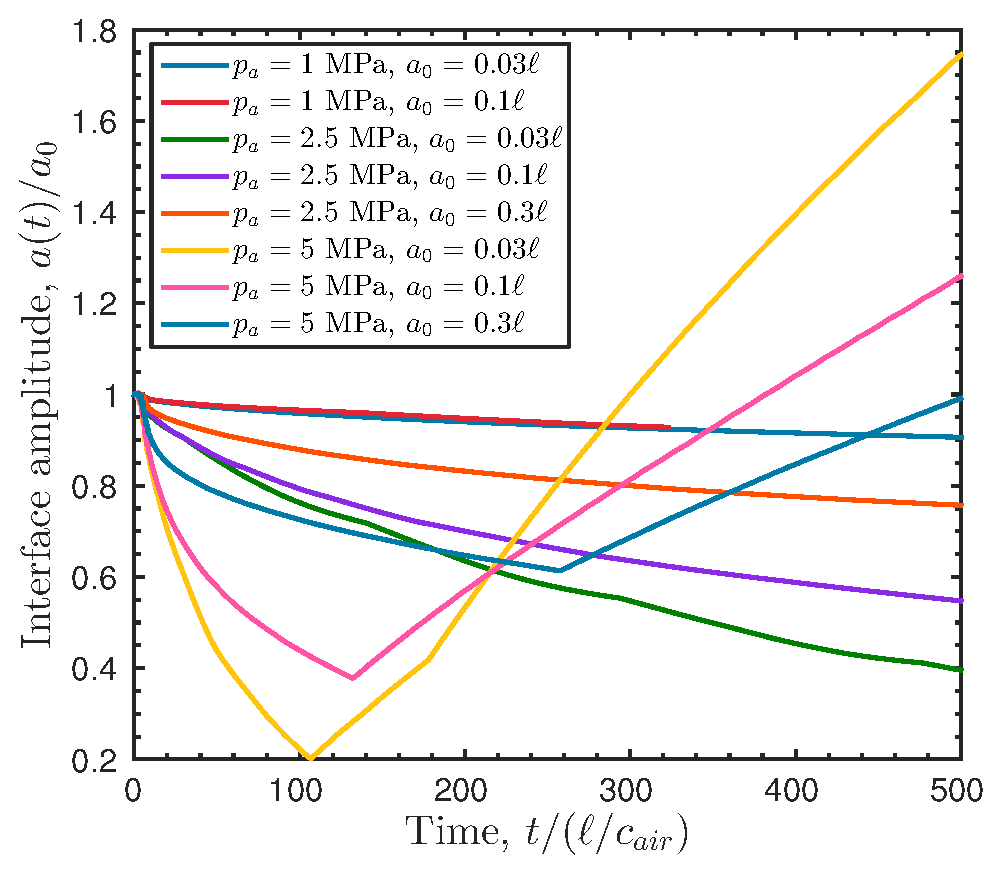
\includegraphics[width=\textwidth]{figs/appendix/rmawave_1_A10,25,50_a03,10,30_Interface_amplitude_02-Mar-2017}
    \caption{Interface amplitude $a(t)$}
  \end{subfigure}
  \begin{subfigure}{0.5\textwidth}
    \centering
    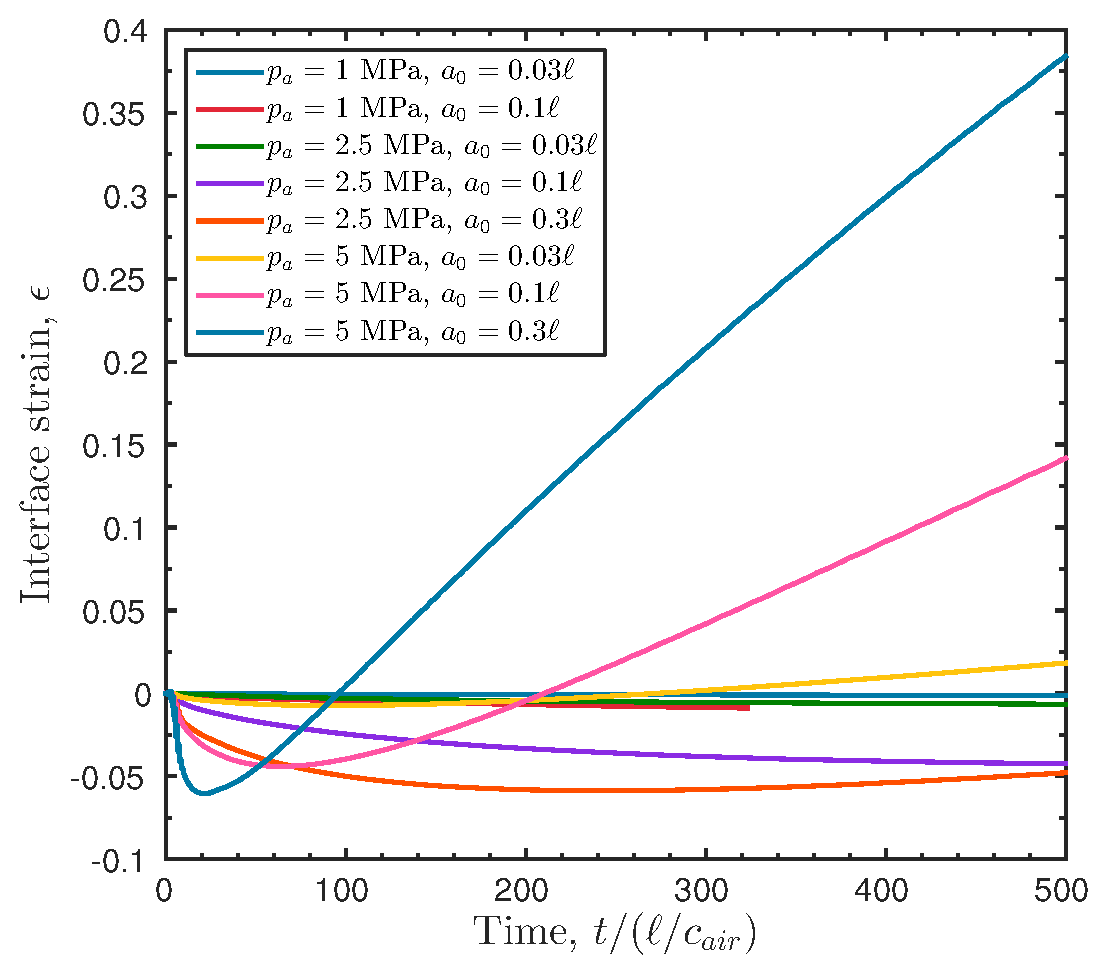
\includegraphics[width=\textwidth]{figs/appendix/rmawave_1_A10,25,50_a3,10,30_epsilon_02-Mar-2017}
    \caption{Strain $\varepsilon(t)$}
  \end{subfigure}
  \begin{subfigure}{\textwidth}
    \centering
    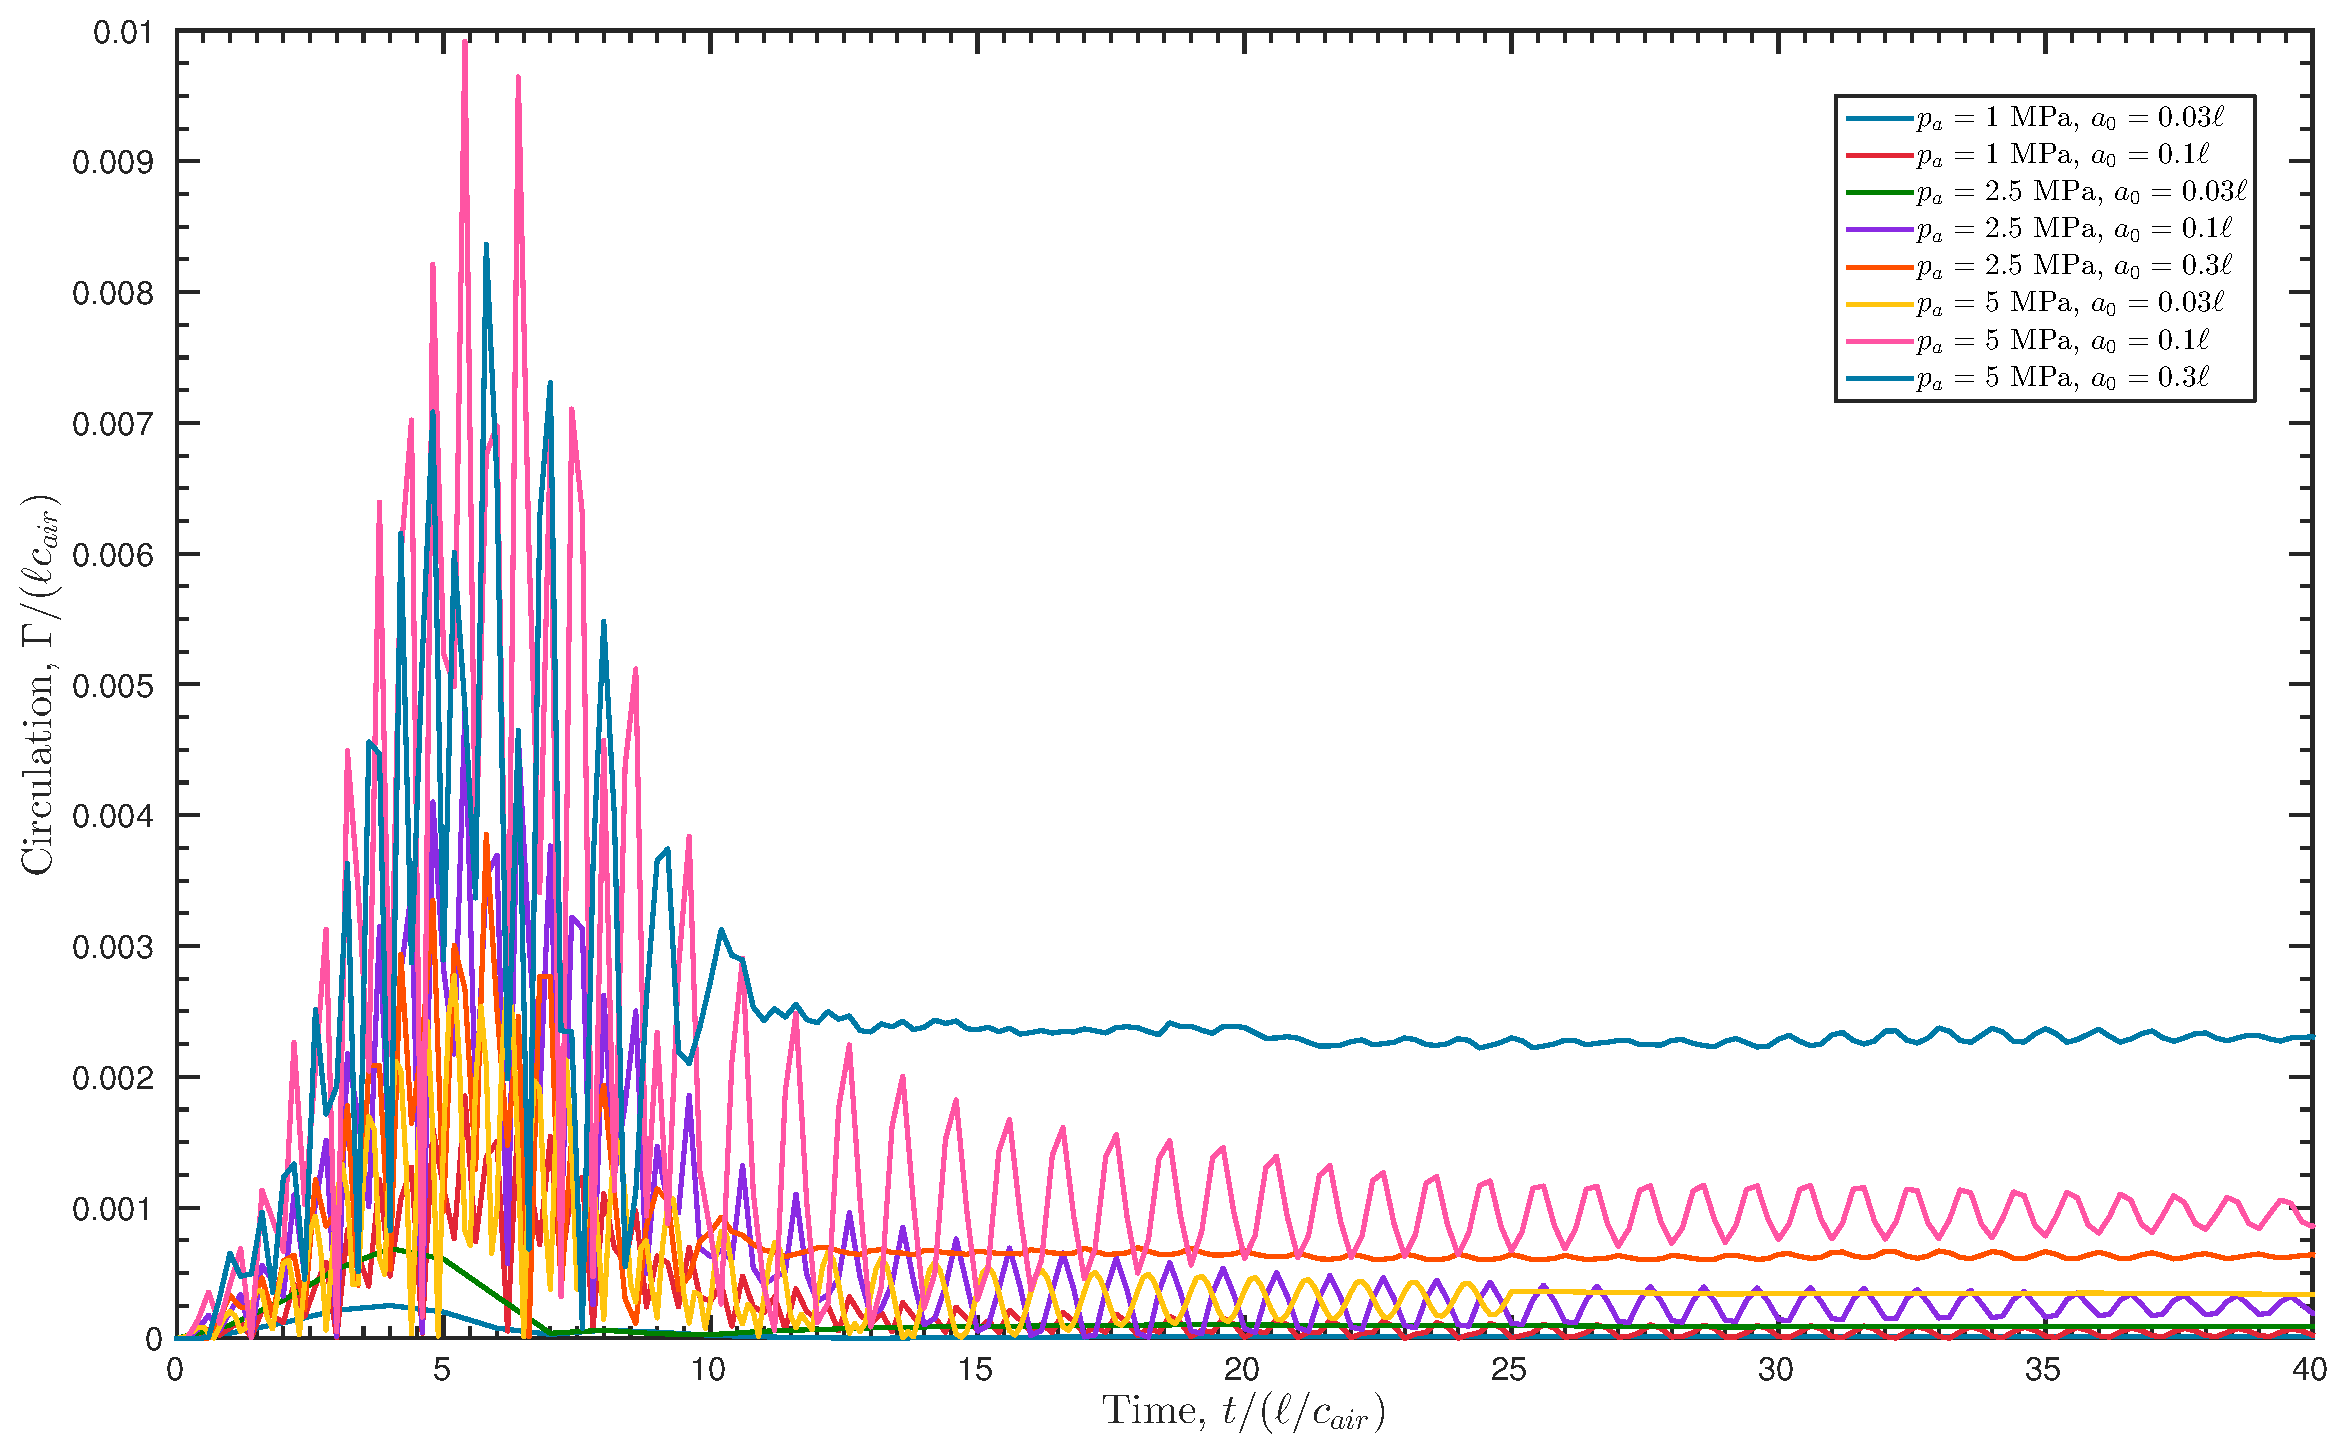
\includegraphics[width=\textwidth]{figs/appendix/rmawave_1_A10,25,50_a03,10,30_circulation_02-Mar-2017}
    \caption{Circulation $\Gamma(t)$}
  \end{subfigure}

  \caption{Interface amplitude, circulation, and strain histories are presented for all ultrasound pulse cases considered in Chapter \ref{ch:usbe_lung_bio}}
\end{figure}

  

%%% Local Variables:
%%% mode: latex
%%% TeX-master: t
%%% End:
